% \iffalse
\let\negmedspace\undefined
\let\negthickspace\undefined
\documentclass[journal,12pt,twocolumn]{IEEEtran}
\usepackage{cite}
\usepackage{amsmath,amssymb,amsfonts,amsthm}
\usepackage{algorithmic}
\usepackage{graphicx}
\usepackage{textcomp}
\usepackage{xcolor}
\usepackage{txfonts}
\usepackage{listings}
\usepackage{enumitem}
\usepackage{mathtools}
\usepackage{gensymb}
\usepackage{comment}
\usepackage[breaklinks=true]{hyperref}
\usepackage{tkz-euclide}
\usepackage{listings}
\usepackage{gvv}
\def\inputGnumericTable{}
\usepackage[latin1]{inputenc}
\usepackage{color}
\usepackage{array}
\usepackage{longtable}
\usepackage{calc}
\usepackage{multirow}
\usepackage{hhline}
\usepackage{ifthen}
\usepackage{lscape}

\newtheorem{theorem}{Theorem}[section]
\newtheorem{problem}{Problem}
\newtheorem{proposition}{Proposition}[section]
\newtheorem{lemma}{Lemma}[section]
\newtheorem{corollary}[theorem]{Corollary}
\newtheorem{example}{Example}[section]
\newtheorem{definition}[problem]{Definition}
\newcommand{\BEQA}{\begin{eqnarray}}
\newcommand{\EEQA}{\end{eqnarray}}
\newcommand{\define}{\stackrel{\triangle}{=}}
\theoremstyle{remark}
\newtheorem{rem}{Remark}
\begin{document}

\bibliographystyle{IEEEtran}
\vspace{3cm}

\title{GATE 2022  -AE 63}
\author{EE23BTECH11057 - Shakunaveti Sai Sri Ram Varun$^{}$% &lt;-this % stops a space
}
\maketitle
\newpage
\bigskip
\vspace{2cm}
\textbf{Question: }
For the circuit shown, the locus of the impedance $ Z\brak{j\omega}$ is plotted as $ \omega$ increases from zero to infinity. The values of $ R_1$ and $ R_2$ are:
\begin{enumerate}
    \item[(A)] $ R_1 = 2\text{ k\ohm}, R_2 = 3\text{ k\ohm}$
    \item[(B)]$ R_1 = 5\text{ k\ohm}, R_2 = 2\text{ k\ohm}$
    \item[(C)] $ R_1 = 5\text{ k\ohm}, R_2 = 2.5\text{ k\ohm}$
    \item[(D)] $ R_1 = 2\text{ k\ohm}, R_2 = 5\text{ k\ohm}$
\end{enumerate}

\begin{figure}[h!]
    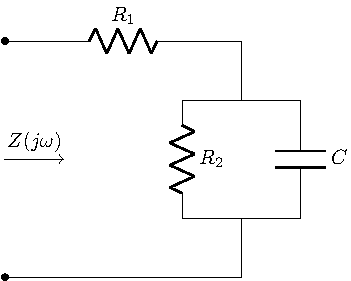
\includegraphics[width = 0.6\columnwidth]{figs/qn_fig.pdf}
    \caption{Figure of circuit}
    \centering
    \label{fig: qn_fig}
\end{figure}

\begin{figure}[h!]
    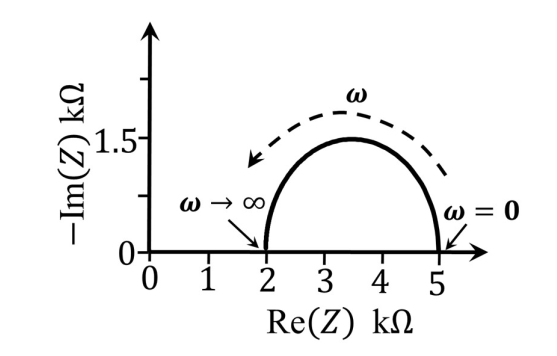
\includegraphics[width = 0.6\columnwidth]{figs/fig_2.png}
    \caption{}
    \centering
    \label{fig: qn_2_fig}
\end{figure}
\hfill(GATE ECE 2022 QUESTION 38)\\
\textbf{Solution}:\\
\begin{table}[h!] 
\centering
\begin{tabular}{|c|c|c|}
    \hline
    \textbf{Parameter} & \textbf{Description} & \textbf{Value} \\
    \hline
    $X\brak{s}$ & position in laplace domain & $ X\brak{s}$ \\
    \hline
    $\Theta\brak{s}$ & angle rotated in laplace domain & $ \Theta\brak{s}$ \\
    \hline
    $x\brak{t}$ & position of mass w.r.t time & $x\brak{t}$ \\
    \hline
    $\theta\brak{t}$ & angle rotated by mass w.r.t time &$ \theta\brak{t}$\\
    \hline
    $\alpha\brak{t}$ & angular acceleration of mass w.r.t time & $\alpha\brak{t}$ \\
    \hline
    $k$ & spring constant & $ k$\\
    \hline
    $m$ & mass of the block & $ m$\\
    \hline
    $L$ & length of the mass & $ L$\\
    \hline
    $\omega_o$ & initial angular velocity of mass & $ \omega_o$ \\
    \hline
    $v\brak{0}$ & initial velocity of mass& $ v\brak{0}$ \\
    \hline
    
\end{tabular}






\caption{input values}
\label{tab: Table2022ECE38}
\end{table}
In $ \omega$ domain (i.e. after Laplace transform) \figref{fig: qn_fig} can be represented as \figref{fig: ans_1_fig}
\begin{figure}[h!]
    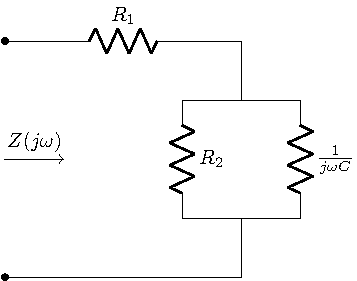
\includegraphics[width = 0.6\columnwidth]{figs/answer_fig.pdf}
    \caption{}
    \centering
    \label{fig: ans_1_fig}
\end{figure}
So, the impedance for the circuit in $ \omega$ domain is:
\begin{align}
Z\brak{j \omega} &= R_1 +  \frac{1}{\frac{1}{R_2}+ j\omega C} \label{eq: ece38_1}
\end{align}
From \figref{fig: qn_2_fig}, $ Z\brak{j\omega}=2$ as $ \omega \to \infty$ and 
$ Z\brak{j\omega}=5$ as $ \omega \to 0$
\begin{align}
2 &= R_1 + \frac{1}{\frac{1}{R_2}+ j\infty}\\
\implies 2\text{\ohm} &= R_1 \label{eq: ece382}\\
5 &= R_1 + \frac{1}{\frac{1}{R_2}+0}\\
\implies 3\text{\ohm} &= R_2
\end{align}
Hence, option (A) is correct.
\end{document}

